\chapter{Implementacja systemu}


\section{Strona internetowa}

Zaprojektowana strona internetowa składa z prostego formularza.
Na stronie został umieszczony przycisk, który umożliwia wybranie zdjęcia z dysku urządzenia klienta.
Po wybraniu zdjęcia pojawia się jego podgląd, po czym plik jest wysyłany na serwer.
Po uzyskaniu odpowiedzi z serwera zostanie wyświetlony otrzymany tekst~\ref{fig:ja}.

\begin{figure}[H]
    \centering
    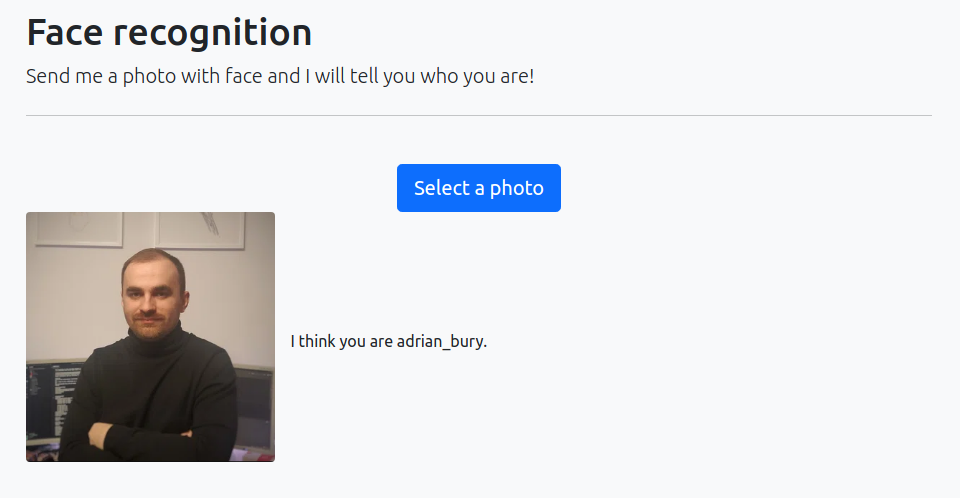
\includegraphics[width=1\textwidth]{./images/wyglad_frontowa_aplikacji}
    \caption{Wygląd strony internetowej po wybraniu zdjęcia z dysku}
    \customsource
    \label{fig:ja}
\end{figure}